\documentclass[11pt, a4paper]{article}

\usepackage{amsmath, amssymb, titling}
\usepackage[margin=2.5cm]{geometry}
\usepackage[colorlinks=true, linkcolor=black, urlcolor=black, citecolor=black]{hyperref}
\usepackage{graphicx}
\usepackage{caption}
\usepackage{subcaption}
\usepackage{float}
\usepackage{cancel}
\usepackage{fancyhdr, lastpage}
\usepackage{fourier-orns}
\usepackage{xcolor}
\usepackage{nomencl}
\makenomenclature

\setlength{\headheight}{18.2pt}

\renewcommand\maketitlehooka{\null\mbox{}\vfill}
\renewcommand\maketitlehookd{\vfill\null}

\renewcommand{\headrule}{
\vspace{-5pt}\hrulefill
\raisebox{-2.1pt}{\quad\leafleft\decoone\leafright\quad}\hrulefill}

\title{Computational Fluid Dynamics \\ HW2}
\author{Almog Dobrescu\\\\ID 214254252}

\pagestyle{fancy}
\cfoot{Page \thepage\ of \pageref{LastPage}}

\begin{document}

\maketitle
\thispagestyle{empty}
\newpage

\thispagestyle{empty}
\tableofcontents
\vfil
\listoffigures
\newpage

\thispagestyle{empty}
\printnomenclature
\newpage

\setcounter{page}{1}
\section{Problem Definition}
\subsection{Governing Equations}
Consider the one-dimensional Navier-Stokes Equations:
\begin{equation}
    \frac{\partial Q}{\partial t}+\frac{\partial E}{\partial x}=\frac{\partial E_v}{\partial x}
\end{equation}
\nomenclature{$Q$}{conservation state space}
\nomenclature{$t$}{time}
\nomenclature{$E$}{inviscid convective vector}
\nomenclature{$E_v$}{viscous convective vector}
\nomenclature{$x$}{spatial coordinate}
Where:
\begin{equation}
    \begin{array}{c}
        \begin{matrix}
            Q=\begin{Bmatrix}
                \rho \\\\
                \rho u \\\\
                e
            \end{Bmatrix}, & E=\begin{Bmatrix}
                \rho u \\\\
                p+\rho u^2 \\\\
                \left(e+p\right)u
            \end{Bmatrix}, & E_v=\begin{Bmatrix}
                0 \\\\
                \displaystyle\frac{4}{3}\mu\frac{\partial u}{\partial x} \\\\
                \displaystyle\frac{4}{3}\mu u\frac{\partial u}{\partial x}-\kappa\frac{\partial T}{\partial x}
            \end{Bmatrix}
        \end{matrix} \\\\
        \begin{matrix}
            \displaystyle p=\left(\gamma-1\right)\left(e-\frac{1}{2}\rho u^2\right), & \displaystyle T=\frac{p}{\rho R}, \\\\
            \displaystyle\mu=1.458\cdot10^{-6}\frac{T^{\frac{3}{2}}}{T+110.4}, & \displaystyle\mu=2.495\cdot10^{-3}\frac{T^{\frac{3}{2}}}{T+194}
        \end{matrix}
    \end{array}
\end{equation}
\nomenclature{$\rho$}{fluid density}
\nomenclature{$u$}{fluid velocity}
\nomenclature{$e$}{total energy}
\nomenclature{$p$}{pressure}
\nomenclature{$\gamma$}{ratio of specific heats}
\nomenclature{$T$}{temperature}
\nomenclature{$R$}{gas constant}
\nomenclature{$\mu$}{coefficient of viscodity}
\nomenclature{$\kappa$}{coefficient of thermal conductivity}
The constants are:
\begin{itemize}
    \item $\gamma=1.4$ for air under standard atmospheric conditions
    \item $R=287.0$ for air
\end{itemize}

\subsection{Physical Domain}
The physical domain is a tube extended between $x=0.2$ and $x=1.0$. At both ends there are impermeable walls.

\subsection{Initial Conditions}
The initial conditions are showen in Fig.\ref{fig: initial conditions}:
\begin{figure}[H]
    \centering
    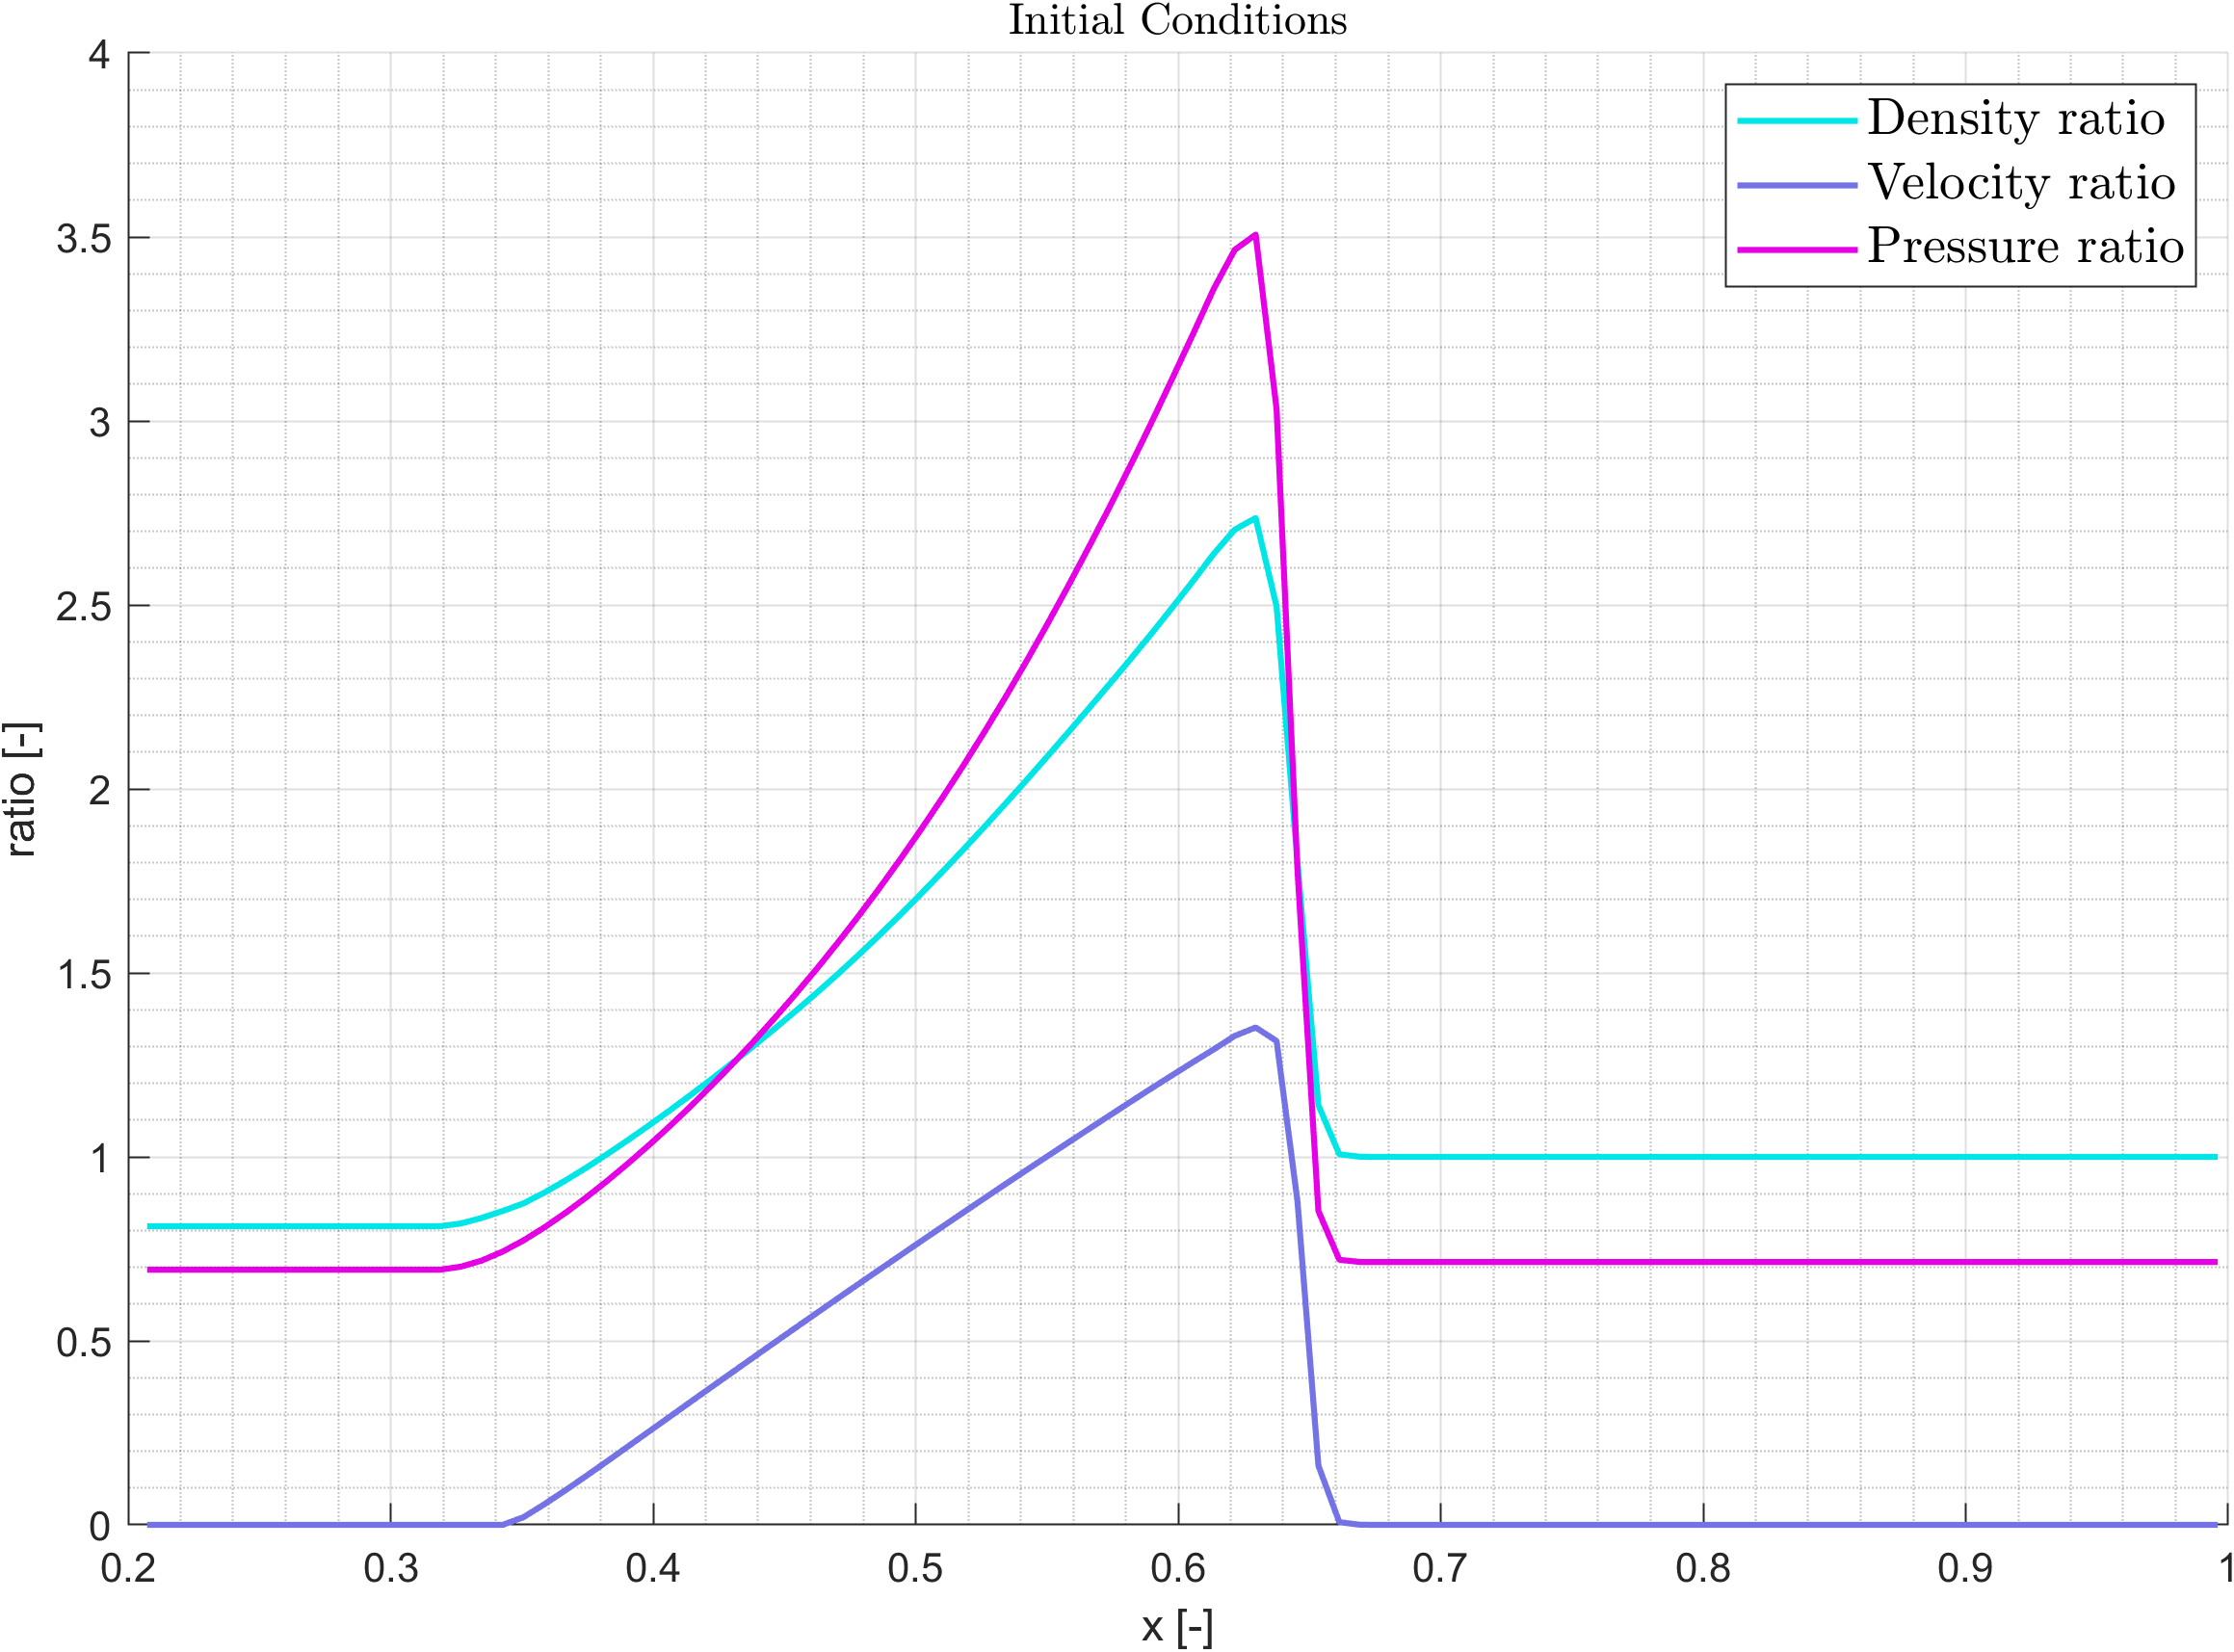
\includegraphics[width=0.5\textwidth]{images/Initial Conditions.png}
    \caption{Initial conditions}
    \label{fig: initial conditions}
\end{figure}

\subsection{Boundary Conditions}
On each side of the tube there is an adiabatic, soild wall boundary conditions. 

\section{The Numerical Shemes}

\newpage
a
\newpage
b

\end{document}